\section{Konzept}\label{sec:konzept}
Anhand der Umfrage wurde ein Konzept für ein Sprachassistenten entwickelt. Dabei wurden die Kosten für benötigte Ressourcen erstmal vernachlässigt. Eine wichtige Anforderung an das Konzept ist der Datenschutz. Die Entwurfsprinzipien für die mehrseitige Sicherheit von Daten nach Kai Rannenberg stellt folgende vier Punkte in den Vordergrund \cite{kairannenberg}:

\begin{enumerate}
	\item Datensparsamkeit
	\item Kontrollmöglichkeiten für den Nutzer 
	\item Auswahlmöglichkeiten und Verhandlungsspielräume 
	\item Dezentralisierung und Verteilung
\end{enumerate} 

Im Rahmen dieses Konzepts wird sich auf die ersten drei Punkte fokussiert. Oftmals erfassen Anwendungen Daten eines Nutzers, die nicht zur Verbesserung der Anwendungen sondern zur Analyse des Nutzer und Weiterverkauf verwendet werden. Deshalb sollt durch das Konzept sichergestellt werden, dass eine Anwendung nur Daten eines Nutzers bezieht, die sie auch tatsächlich benötigt. Des Weiteren sollen die erfassten Daten dem Nutzer transparent dargestellt werden. Somit kann der Nutzer seine erfassten Daten auch manipulieren bzw. anonymisieren. 

Damit soll der zu entwickelnde Sprachassistent folgende Anforderungen erfüllen:
\begin{itemize}
	\item User-Controlled-Privacy
	\item Funktionalität
	\item Performance
	\item Nutzerfreundlichkeit	
\end{itemize}

Durch User-Controlled Privacy kann ein Nutzer bestimmen, welche Daten er von sich für eine bestimmte Anwendungen freigibt. Anwendungen benötigen jedoch auch Daten eines Nutzers, denn dadurch können diese Nutzerfreundlichkeit bieten. Ein Beispiel ist die Frage eines Sprachassistenten nach der Wettervorhersage. Weiß der Sprachassistent wo sich ein Nutzer gerade befindet, so kann dieser direkt die Wettervorhersage für die aktuelle Position des Nutzer liefern. Anderseits muss der Sprachassistent zuerst den Nutzer Fragen, für welchen Ort dieser eine Wettervorhersage haben will. Will ein Nutzer seine Daten für eine Anwendungen nicht freigeben, so kann er einen fiktiven Kontext von sich angeben. Dadurch kann der Nutzer die Anwendungen trotzdem  auf Kosten von Nutzerfreundlichkeit nutzen.

Ein Kontext beschreibt die Eigenschaften eines Nutzers, welche Attribute ein Kontext hat, wird in Abbildung \ref{fig:kontext} dargestellt. In dem Beispielszenario \glqq Hobby Benachrichtigung \grqq{} kann der Kontext genutzt werden, um ein Nutzer mögliche Termine für Ausübungen seines Hobbys vorzuschlagen. Beispielsweise kann anhand des Kontexts des Nutzers der Kalender, der Wetterbericht für dessen Standort und dessen Hobbys ermittelt werden. 

\begin{figure}[!h]
	\centering
	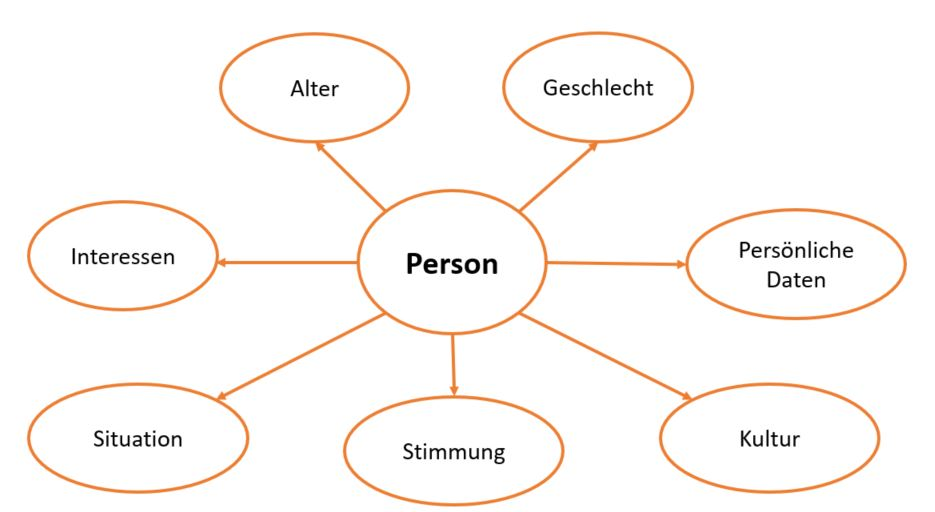
\includegraphics[width=1\linewidth]{Picture/Kontext}
	\caption[Nuzter Kontext]{Nuzter Kontext}
	\label{fig:kontext}
\end{figure}





